\documentclass[tikz,border=10pt]{standalone}
% Coordinates in cm, origin at C (scale ~0.0147 cm per px, y up)
\begin{document}
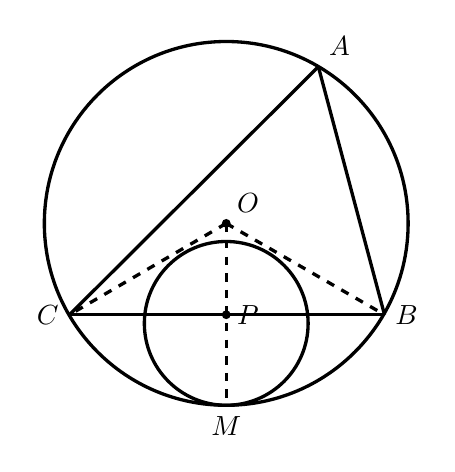
\begin{tikzpicture}[line width=1.2pt, line join=round]
  % Key points
  \coordinate (C) at (0,0);
  \coordinate (B) at (4.00,0);
  \coordinate (A) at (3.16,3.15);
  \coordinate (O) at (1.99,1.16);
  \coordinate (P) at (1.99,0);
  \coordinate (M) at (1.99,-1.15);
  \coordinate (S) at (1.99,-0.11);   % centre of small circle

  % Large circle centred at O through A, B, C, M
  \draw (O) circle[radius=2.31];

  % Small circle tangent internally at M
  \draw (S) circle[radius=1.04];

  % Solid chords
  \draw (A) -- (C);
  \draw (A) -- (B);
  \draw (C) -- (B);

  % Dashed radii OC, OB and vertical OM
  \draw[dashed] (O) -- (C);
  \draw[dashed] (O) -- (B);
  \draw[dashed] (O) -- (M);

  % Dots at O and P
  \fill (O) circle[radius=1.6pt];
  \fill (P) circle[radius=1.6pt];

  % Labels
  \node[above right] at (A) {$A$};
  \node[right] at (B) {$B$};
  \node[left] at (C) {$C$};
  \node[above right] at (O) {$O$};
  \node[right] at (P) {$P$};
  \node[below] at (M) {$M$};
\end{tikzpicture}
\end{document}